%%%
%
% $Autor: Wings $
% $Datum: 2021-05-14 $
% $Pfad: GitLab/MLEdgeComputer $
% $Dateiname: AdapterBoard
% $Version: 4620 $
%
% !TeX spellcheck = de_DE/GB
% !TeX program = pdflatex
% !BIB program = biber/bibtex
% !TeX encoding = utf8
%
%%%



\chapter{Terminal Adapter Board mit Schraubklemmen kompatibel mit Nano V3 und Arduino}

Das verwendete Shield führt alle Anschlüsse des Arduinos auf außenliegende Schraubklemmen. Dies ermöglicht die Nutzung aller Anschlüsse durch das Verwenden von Jumper-Kabeln. Das Shield ist in der folgenden Abbildung \ref{fig:shield} zu sehen. Die Abmessungen des Shields sind 54x43x13mm und es hat ein Gewicht von 21 Gramm. \cite{AZ-Delivery:2024}

\begin{figure}
    \centering
    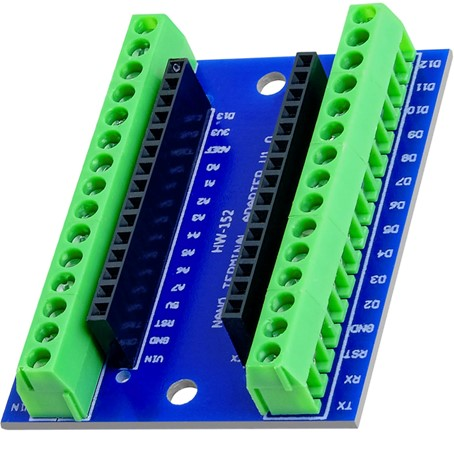
\includegraphics [width=70mm] {AdapterBoard/shield}
    \caption{Terminal Adapter Board mit Schraubklemmen kompatibel mit Nano V3 und Arduino}
    \label{fig:shield}
\end{figure}
